

\tikzset{every picture/.style={line width=0.75pt}} %set default line width to 0.75pt

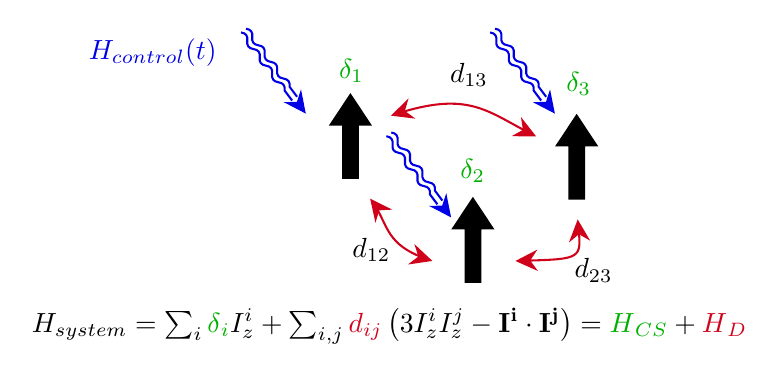
\begin{tikzpicture}[x=0.75pt,y=0.75pt,yscale=-1,xscale=1]
%uncomment if require: \path (0,321); %set diagram left start at 0, and has height of 321

%Up Arrow [id:dp3616533286619681]
\draw  [fill={rgb, 255:red, 0; green, 0; blue, 0 }  ,fill opacity=1 ] (156,55.33) -- (165.5,41) -- (175,55.33) -- (169.03,55.33) -- (169.03,81) -- (161.97,81) -- (161.97,55.33) -- cycle ;
%Up Arrow [id:dp5012912754811447]
\draw  [fill={rgb, 255:red, 0; green, 0; blue, 0 }  ,fill opacity=1 ] (215,105.33) -- (224.5,91) -- (234,105.33) -- (228.03,105.33) -- (228.03,131) -- (220.97,131) -- (220.97,105.33) -- cycle ;
%Up Arrow [id:dp52188591349806]
\draw  [fill={rgb, 255:red, 0; green, 0; blue, 0 }  ,fill opacity=1 ] (265,65.33) -- (274.5,51) -- (284,65.33) -- (278.03,65.33) -- (278.03,91) -- (270.97,91) -- (270.97,65.33) -- cycle ;
%Curve Lines [id:da4574392367290909]
\draw [color={rgb, 255:red, 208; green, 2; blue, 27 }  ,draw opacity=1 ]   (176.84,93.56) .. controls (183.95,104.28) and (182.51,113.13) .. (202.4,120.13) ;
\draw [shift={(205,121)}, rotate = 197.49] [fill={rgb, 255:red, 208; green, 2; blue, 27 }  ,fill opacity=1 ][line width=0.08]  [draw opacity=0] (10.72,-5.15) -- (0,0) -- (10.72,5.15) -- (7.12,0) -- cycle    ;
\draw [shift={(175,91)}, rotate = 51.91] [fill={rgb, 255:red, 208; green, 2; blue, 27 }  ,fill opacity=1 ][line width=0.08]  [draw opacity=0] (10.72,-5.15) -- (0,0) -- (10.72,5.15) -- (7.12,0) -- cycle    ;
%Curve Lines [id:da7885055809075856]
\draw [color={rgb, 255:red, 208; green, 2; blue, 27 }  ,draw opacity=1 ]   (248.47,120.9) .. controls (277.46,120.07) and (276.79,119.99) .. (275.27,103.96) ;
\draw [shift={(275,101)}, rotate = 445.16] [fill={rgb, 255:red, 208; green, 2; blue, 27 }  ,fill opacity=1 ][line width=0.08]  [draw opacity=0] (10.72,-5.15) -- (0,0) -- (10.72,5.15) -- (7.12,0) -- cycle    ;
\draw [shift={(245,121)}, rotate = 358.33] [fill={rgb, 255:red, 208; green, 2; blue, 27 }  ,fill opacity=1 ][line width=0.08]  [draw opacity=0] (10.72,-5.15) -- (0,0) -- (10.72,5.15) -- (7.12,0) -- cycle    ;
%Curve Lines [id:da5782733153480035]
\draw [color={rgb, 255:red, 208; green, 2; blue, 27 }  ,draw opacity=1 ]   (188.37,49.9) .. controls (222.59,39.07) and (231.43,48.94) .. (252.64,59.81) ;
\draw [shift={(255,61)}, rotate = 206.24] [fill={rgb, 255:red, 208; green, 2; blue, 27 }  ,fill opacity=1 ][line width=0.08]  [draw opacity=0] (10.72,-5.15) -- (0,0) -- (10.72,5.15) -- (7.12,0) -- cycle    ;
\draw [shift={(185,51)}, rotate = 341.27] [fill={rgb, 255:red, 208; green, 2; blue, 27 }  ,fill opacity=1 ][line width=0.08]  [draw opacity=0] (10.72,-5.15) -- (0,0) -- (10.72,5.15) -- (7.12,0) -- cycle    ;

%Straight Lines [id:da5939121577594202]
\draw [color={rgb, 255:red, 0; green, 0; blue, 231 }  ,draw opacity=1 ]   (115.2,9.1) .. controls (117.53,9.43) and (118.53,10.77) .. (118.2,13.1) .. controls (117.87,15.43) and (118.87,16.77) .. (121.2,17.1) .. controls (123.53,17.43) and (124.53,18.77) .. (124.2,21.1) .. controls (123.87,23.43) and (124.87,24.77) .. (127.2,25.1) .. controls (129.53,25.43) and (130.53,26.77) .. (130.2,29.1) .. controls (129.87,31.43) and (130.87,32.77) .. (133.2,33.1) .. controls (135.53,33.43) and (136.53,34.77) .. (136.2,37.1) -- (138,39.5) -- (139.8,41.9)(112.8,10.9) .. controls (115.13,11.23) and (116.13,12.57) .. (115.8,14.9) .. controls (115.47,17.23) and (116.47,18.57) .. (118.8,18.9) .. controls (121.13,19.23) and (122.13,20.57) .. (121.8,22.9) .. controls (121.47,25.23) and (122.47,26.57) .. (124.8,26.9) .. controls (127.13,27.23) and (128.13,28.57) .. (127.8,30.9) .. controls (127.47,33.23) and (128.47,34.57) .. (130.8,34.9) .. controls (133.13,35.23) and (134.13,36.57) .. (133.8,38.9) -- (135.6,41.3) -- (137.4,43.7) ;
\draw [shift={(144,50)}, rotate = 233.13] [fill={rgb, 255:red, 0; green, 0; blue, 231 }  ,fill opacity=1 ][line width=0.08]  [draw opacity=0] (10.72,-5.15) -- (0,0) -- (10.72,5.15) -- (7.12,0) -- cycle    ;
%Straight Lines [id:da5935560230770542]
\draw [color={rgb, 255:red, 0; green, 0; blue, 231 }  ,draw opacity=1 ]   (235.2,9.1) .. controls (237.53,9.43) and (238.53,10.77) .. (238.2,13.1) .. controls (237.87,15.43) and (238.87,16.77) .. (241.2,17.1) .. controls (243.53,17.43) and (244.53,18.77) .. (244.2,21.1) .. controls (243.87,23.43) and (244.87,24.77) .. (247.2,25.1) .. controls (249.53,25.43) and (250.53,26.77) .. (250.2,29.1) .. controls (249.87,31.43) and (250.87,32.77) .. (253.2,33.1) .. controls (255.53,33.43) and (256.53,34.77) .. (256.2,37.1) -- (258,39.5) -- (259.8,41.9)(232.8,10.9) .. controls (235.13,11.23) and (236.13,12.57) .. (235.8,14.9) .. controls (235.47,17.23) and (236.47,18.57) .. (238.8,18.9) .. controls (241.13,19.23) and (242.13,20.57) .. (241.8,22.9) .. controls (241.47,25.23) and (242.47,26.57) .. (244.8,26.9) .. controls (247.13,27.23) and (248.13,28.57) .. (247.8,30.9) .. controls (247.47,33.23) and (248.47,34.57) .. (250.8,34.9) .. controls (253.13,35.23) and (254.13,36.57) .. (253.8,38.9) -- (255.6,41.3) -- (257.4,43.7) ;
\draw [shift={(264,50)}, rotate = 233.13] [fill={rgb, 255:red, 0; green, 0; blue, 231 }  ,fill opacity=1 ][line width=0.08]  [draw opacity=0] (10.72,-5.15) -- (0,0) -- (10.72,5.15) -- (7.12,0) -- cycle    ;
%Straight Lines [id:da7272100103209711]
\draw [color={rgb, 255:red, 0; green, 0; blue, 231 }  ,draw opacity=1 ]   (185.2,59.1) .. controls (187.53,59.43) and (188.53,60.77) .. (188.2,63.1) .. controls (187.87,65.43) and (188.87,66.77) .. (191.2,67.1) .. controls (193.53,67.43) and (194.53,68.77) .. (194.2,71.1) .. controls (193.87,73.43) and (194.87,74.77) .. (197.2,75.1) .. controls (199.53,75.43) and (200.53,76.77) .. (200.2,79.1) .. controls (199.87,81.43) and (200.87,82.77) .. (203.2,83.1) .. controls (205.53,83.43) and (206.53,84.77) .. (206.2,87.1) -- (208,89.5) -- (209.8,91.9)(182.8,60.9) .. controls (185.13,61.23) and (186.13,62.57) .. (185.8,64.9) .. controls (185.47,67.23) and (186.47,68.57) .. (188.8,68.9) .. controls (191.13,69.23) and (192.13,70.57) .. (191.8,72.9) .. controls (191.47,75.23) and (192.47,76.57) .. (194.8,76.9) .. controls (197.13,77.23) and (198.13,78.57) .. (197.8,80.9) .. controls (197.47,83.23) and (198.47,84.57) .. (200.8,84.9) .. controls (203.13,85.23) and (204.13,86.57) .. (203.8,88.9) -- (205.6,91.3) -- (207.4,93.7) ;
\draw [shift={(214,100)}, rotate = 233.13] [fill={rgb, 255:red, 0; green, 0; blue, 231 }  ,fill opacity=1 ][line width=0.08]  [draw opacity=0] (10.72,-5.15) -- (0,0) -- (10.72,5.15) -- (7.12,0) -- cycle    ;


% Text Node
\draw (10.5,142.4) node [anchor=north west][inner sep=0.75pt]    {$H_{\text{system}} =\sum _{i}\textcolor[rgb]{0,0.69,0}{\delta }\textcolor[rgb]{0,0.69,0}{_{i}} I^{i}_{z} +\sum _{i,j}\textcolor[rgb]{0.82,0.01,0.11}{d}\textcolor[rgb]{0.82,0.01,0.11}{_{ij}}\left( 3I^{i}_{z} I^{j}_{z} -\mathbf{I^{i}} \cdot \mathbf{I^{j}}\right) =\textcolor[rgb]{0,0.69,0}{H}\textcolor[rgb]{0,0.69,0}{_{\text{CS}}} +\textcolor[rgb]{0.82,0.01,0.11}{H}\textcolor[rgb]{0.82,0.01,0.11}{_{D}}$};
% Text Node
\draw (165,108.4) node [anchor=north west][inner sep=0.75pt]  [font=\normalsize]  {$d_{12}$};
% Text Node
\draw (272,118.4) node [anchor=north west][inner sep=0.75pt]  [font=\normalsize]  {$d_{23}$};
% Text Node
\draw (212,24.4) node [anchor=north west][inner sep=0.75pt]  [font=\normalsize]  {$d_{13}$};
% Text Node
\draw (158.5,22.4) node [anchor=north west][inner sep=0.75pt]  [color={rgb, 255:red, 0; green, 175; blue, 0 }  ,opacity=1 ]  {$\delta _{1}$};
% Text Node
\draw (217,70.4) node [anchor=north west][inner sep=0.75pt]  [color={rgb, 255:red, 0; green, 175; blue, 0 }  ,opacity=1 ]  {$\delta _{2}$};
% Text Node
\draw (268,28.4) node [anchor=north west][inner sep=0.75pt]  [color={rgb, 255:red, 0; green, 175; blue, 0 }  ,opacity=1 ]  {$\delta _{3}$};
% Text Node
\draw (38,12.4) node [anchor=north west][inner sep=0.75pt]  [color={rgb, 255:red, 0; green, 0; blue, 231 }  ,opacity=1 ]  {$H_{\text{control}}( t)$};


\end{tikzpicture}
